%!TEX=xlatex
\documentclass[UTF-8,AutoFakeBold]{article}%支持粗体
\usepackage{ctex}
\usepackage{soul}
\usepackage{color}
\usepackage{geometry}   % 页边距调整
\usepackage{setspace}   % 行距调整
\usepackage{graphicx}   % 图片支持
\usepackage{float}      % 图片强制放置
\usepackage{xcolor}     % 代码着色
\usepackage{listings}   % 代码支持
\usepackage{indentfirst}% 首行缩进
\usepackage{titlesec}   % 设置标题
\usepackage{zhnumber}   % 设置中文section序号
\usepackage{amsmath,amssymb}    % 数学公式
\usepackage{fancyhdr}
\usepackage{siunitx}
\usepackage{enumerate}
\usepackage{booktabs}
\usepackage{subcaption}
\usepackage{pgfplots}
% 页边距调整
\geometry{
	a4paper,
	left=2.54cm,
	right=1.5cm,
	top=1cm,
	bottom=2.54cm
}
% 设置页眉页脚
\pagestyle{fancy}
\fancyhf{} % 清除所有页眉页脚
\renewcommand{\headrulewidth}{0pt} % 去页眉线
\fancyfoot[C]{第 \thepage 页} % 设置页码

% 设置section和subsection
\setcounter{secnumdepth}{4}
\titleformat{\section}{\bfseries}{\Large \chinese{section}、}{0em}{\Large }
\titleformat{\subsection}{\bfseries}{\arabic{subsection}}{0.5em}{}
\titleformat{\subsubsection}{\bfseries}{\arabic{subsection}.\arabic{subsubsection}}{0.5em}{}
\titleformat{\paragraph}{\bfseries}{\arabic{subsection}.\arabic{subsubsection}.\arabic{paragraph}}{0.5em}{}
\newcommand{\subsubsubsection}{\paragraph}
\titlespacing*{\section}{0pt}{3.5ex}{2.3ex}
\titlespacing*{\subsection}{0pt}{3.25ex}{1.5ex}
\titlespacing*{\subsubsection}{0pt}{3.25ex}{1.5ex}
\titlespacing*{\paragraph}{0pt}{2ex}{1em}
\titlespacing*{\subparagraph}{\parindent}{0.5em}{1em}
% 行距调整
\linespread{1.25}
% 首行缩进
\setlength{\parindent}{2em}


\begin{document}
\begin{figure}[t]
    \centering
    
\includegraphics[width=5cm]{image/zjutag.jpg}
    \textbf{\Huge\heiti 实验报告}
    \qquad\qquad
    \parbox[b]{5cm}{
        专业:\underline{\hbox to 0.75\linewidth{\hfill 1 \hfill}}\\

        \vspace{-1.5ex}
        姓名:\underline{\hbox to 0.75\linewidth{\hfill 1 \hfill}}\\

        \vspace{-1.5ex}
        学号:\underline{\hbox to 0.75\linewidth{\hfill 1 \hfill}}\\

        \vspace{-1.5ex}
        日期:\underline{\hbox to 0.75\linewidth{\hfill 1 \hfill}}\\

        \vspace{-1.5ex}
        地点:\underline{\hbox to 0.75\linewidth{\hfill 1 \hfill}}\\
    }
\end{figure}
\vspace{6ex}
\begin{flushleft}
    \parbox{1\linewidth}{
    \centering
    课程名称:\underline{\hbox to  0.3\linewidth{\hfill 1 \hfill}}
    指导老师:\underline{\hbox to 0.22\linewidth{\hfill 1 \hfill}}
    成绩:   \underline{\hbox to 0.15\linewidth{\hfill 1 \hfill}}\\
    实验名称:\underline{\hbox to  0.3\linewidth{\hfill 1 \hfill}}
    实验类型:\underline{\hbox to 0.22\linewidth{\hfill 1 \hfill}}
    组号:   \underline{\hbox to 0.15\linewidth{\hfill 1 \hfill}}\\
    
}
\end{flushleft}


\begin{flushleft} 
    \centering
    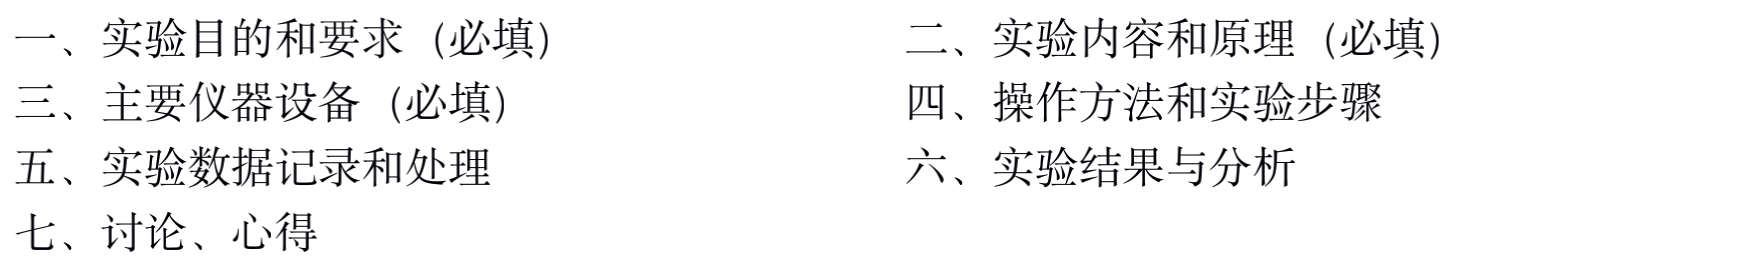
\includegraphics[width=1.2\linewidth]{image/zju_content.png}
\end{flushleft}
\vspace*{6ex}

\section{实验目的和要求}
\subsection{s}
asdf
\subsubsection{ss}
\subsubsubsection{sss}
\subsection*{s}
\subsubsection*{ss}
\subsubsubsection*{sss}
\section{实验内容和原理}

\section{主要实验仪器}

\section{操作方法及实验步骤}

\section{实验数据记录和处理}

\section{实验结果与分析}

\section{讨论、心得}

\end{document}